% chap1.tex {Introductory Chapter}

\chapter{Introduction}
\section{Training a Neural Network}
A neural network is a function $f(\bm{x};\bm{\theta})$ that maps an input $\bm{x}$ to some response variable $y$. When we \textit{train} a
neural network, we \textit{learn} the model parameters, or weights, $\bm{\theta}$ that minimize some cost function $J(\bm{\theta})$.
For a regression task, where the model's output is a continuous variable, a common cost function is the \textbf{Mean Square Error}:
\[J(\theta) = \frac{1}{m}\sum_{i=1}^{m}(y_{i} - f(\bm{x}_{i};\bm{\theta}))^{2}\]

For categorical or discrete output variables found in classification tasks, we normally use the \textbf{Categorical Cross-Entropy}:

\[J(\bm{\theta}) = -\mathbb{E}_{\bm{x},y \sim \hat p_{data}} \log \textit{p}(y|\bm{x};\bm{\theta})\]

Given a \textit{training} set of observations $\bm{x}_i$ and their true labels $y_i$, we compute weights that minimize the cost, or error, via
maximum likelihood (ML) estimation:

\[\bm{\theta}_{ML} = \argmax_{\bm{\theta}} \sum_{i}^{m} \log P(y_{i}|\bm{x}_{i};\bm{\theta})\],

which one can see is equivalent to computing the weights that \textbf{\textit{minimize}} the cross-entropy cost function.


\section{Minimizing Non-Convex Functions: Gradiant-Based Learning}
%Convex functions possess many desireable properties that make optimization easy.
%The global minimum of a strictly convex function without constraint is guaranteed and any local minimum is a global minimum.
%A procedure that optimizes such a function via iterative updates such as coordinate descent is also guaranteed to
%converge from any initial point in parameter space \cite{Luo199}. One familiar example of a convex function is the function
%\[f(x) = x^2\]
%where the global optimum lies at $x=0$.

Due to the non-linearities associated with a neural network, the loss function to be minimized becomes non-convex.
[Elaborate (Weight symmetry, model identifiability, etc)]
Non-convex optimization is in general more difficult than convex optimization, so we usually rely on gradient-based methods for the task.
Gradient based optimization provides a sound theoretical framework and a practical and well tested methodology for learning
deep neural networks. This gradient-based learning process involves \textit{moving},
or updating, the weight values in the direction opposite of the cost function's gradient, repeating this process for a series of
\textbf{epochs}, or training iterations.
These updates should be small, scaled by a
\textit{learning rate}, and can make learning a lengthy process. Gradient based learning is also scalable to datasets of enourmous size.
The gradients and updates may be computed using small random batches of the training set at a time rather than the entire dataset (e.g. Stochastic Gradient Descent) CITE[BOTOU 2010].

\section{Bias-Variance Tradeoff}

Given a set of i.i.d. observations $\{\bm{x}_1, ... , \bm{x}_n\}$, we wish to compute the set of weights $\bm{\hat{\theta}}$ that is as close
as possible to $\bm{\theta}$, the set of weights that truly parametrize the data generating process $p_{data}(\bm{x};\bm{\theta})$.
This concrete parameter value (in contrast to a density over possible values) is called a \textbf{point estimator}, or statistic, of the true
set of parameters.
Unless the data generating process is known exactly the parameter estimators will have error.
Two different measures of error in an estimator are its bias and variance.
The \textbf{bias} measures the expected deviation between $\bm{\theta}$ and the estimator $\bm{\hat{\theta}}$,
this expectation over the data:

\[Bias(\bm{\hat{\theta}}) = \mathbb{E}{(\bm{\hat{\theta}})} - \bm{\theta}\]
\[ = \mathbb{E}{[\bm{\hat{\theta}} - \bm{\theta}}]\]

The \textbf{variance} is a measure of the deviation from the expected estimator, caused by
the randomness in the sample, or how much the estimator will vary as a function of the data sample:

\[ Var(\bm{\hat{\theta}}) = \mathbb{E}{(\bm{\theta} - \bm{\hat{\theta}})^{2}}\]

When learning a neural network's weights, we use a \textit{training set} so that we can later generalize
previously unseen data with high accuracy (or some other determined metric). That means that during training, we
obtain $\bm{\theta}_{ML}$ by minimizing $J_{train}(\bm{\theta})$, but we care about having low $J_{test}(\bm{\theta})$ i.e. low cost
on test data points.

\begin{figure}[h]
\caption{Visualization of overfitting. Training error decreases as epochs progress, eventually reaching zero.
Validation error starts increasing, indicating overfitting. The best model is shown at the dotted line, where
validation error reached its minimum.}
\centering
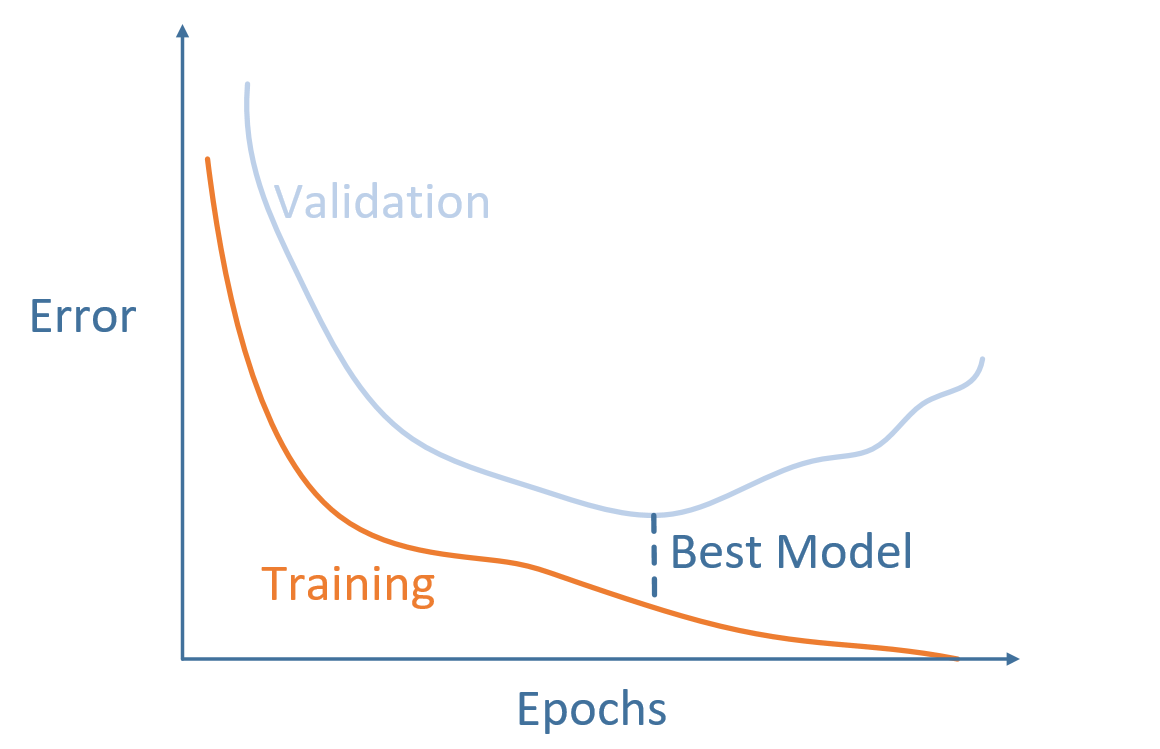
\includegraphics[width=0.5\textwidth]{OverfittingLossPlot.png}
\end{figure}

\textbf{Overfitting} occurs when a network is able to predict its training set extremely well i.e. very close to zero error, but fails to predict
unseen data points. This is because the network's weights have been extremely fine-tuned to \textit{fit} its training data, but do not fit or represent
data points outside of its training samples.
An overfitted model is said to have large \textbf{variance} and small \textbf{bias}. Conversely, underfitting occurs when the model fails to predict
the training set because it generalizes too much. This model is said to have large bias and small variance. When training a neural network,
we aim to find a balance between training cost and test cost, between overfitting and underfitting.

Because of the commonly large number of weights in deep convolutional networks, it is easy to overfit a moderate size training set CITE[HINTON et all 2012].
It has been shown that when using a large enough dataset, neural networks are trained without overfitting, and thus generalize well
to new unseen data. Because of the abundance of data today, it is usually easy to acquire large datasets, although this is not always the case.
In this work, we consider the case then the sizes of available datasets are moderately sized e.g. a tens of thousands.

\section{Weight Regularization}
One way to regularize a model is to impose a constraint on its weights. By adding a penalty term to the cost function, we can decrease the
magnitude of our weights to to prevent them from \textit{blowing up} and overfitting the training set. $\bm{L_2}$ regularization
adds the L2 norm of the weights to the cost function:

\[J(\bm{\theta}) = -\mathbb{E}_{\bm{x},y \sim \hat p_{data}} \log \textit{p}(y|\bm{x};\bm{\theta}) + \lambda \lVert \bm{\theta} \rVert_{2}\]

where $\lambda$ is the regularization control parameter. Higher values of $\lambda$ penalize more and a value of 0 leads to no regularization.

\subsection{Dropout}
A recently proposed and highly effective way to regularize a neural network is via \textbf{dropout}CITE[HINTON et all 2012]CITE[Srivastava et al 2014].
Dropout "deactivates" a neuron or unit with probability $p_{drop}$. We deactivate a unit
by setting its output to 0. This forces the network to not rely on combinations of
activations, since any unit will only be \textit{active} with probability $1-p_{drop}$.
